\documentclass[12pt]{article}


\usepackage[]{fullpage}
\usepackage{graphicx}

\usepackage{natbib}
\usepackage{hyperref}
\usepackage{tabularx}
\usepackage{float}

% Set graphics path
\graphicspath{ {./Images/} }

% Headers and footers https://en.wikibooks.org/wiki/LaTeX/Customizing_Page_Headers_and_Footers
\usepackage{fancyhdr}
\fancyfoot{}
\renewcommand{\headrulewidth}{0pt}
\renewcommand{\footrulewidth}{0pt}
\lhead{CMP-7030Y - Research Techniques}
\rhead{}
\fancyfoot[R]{\thepage}
\fancyfoot[L]{100130020 George Markham}


\title{Topic 22: User identification}
\author{George Markham\\Reg 100130020\\\small
% george.markham@uea.ac.uk}
\href{mailto:george.markham@uea.ac.uk}{george.markham@uea.ac.uk}}

\begin{document}
	\maketitle
	
% 	Make special footer just for title page, without header https://en.wikibooks.org/wiki/LaTeX/Customizing_Page_Headers_and_Footers
	\fancypagestyle{plain}{\fancyhf{}\fancyfoot[R]{\thepage}}
    
	\begin{abstract}
	Due to the increasing amount of sensitive data people entrust to online services it is important that this data is kept secure and only accessible by authorised parties. Usernames \& passwords consistently fail as verification and identification methods therefore alternatives must be considered. This report discusses both biometric and behavioural biometric methods of verification and identification. The methods by which researchers determine their performance is also investigated. This report finds that both biometrics and behavioural biometrics are good candidates for replacing or augmenting username \& password systems and, while biometric identification is likely better in most cases than behavioural biometric identification, for verification tasks behavioural biometrics are both less obtrusive and can work as well as their biometric counterparts.
	\end{abstract}
	
	\tableofcontents
	
    % 	Apply headers
	\pagestyle{fancy}
    \fancypagestyle{plain}{\pagestyle{fancy}}
    \setlength{\headsep}{1cm}
    
	\section{Introduction}
	User identification has become increasingly important with the advent of the internet. Businesses, governments, and the general public are sharing personal, sometimes very sensitive information with trusted parties. The key issue being that word \emph{`trusted'}. How does one prove one's identity to another user or system across the globe? 
	
	There are seemingly constantly news stories relating to data theft, last year's Equifax (credit reporting agency) hack could have potentially leaked nearly half the population of the United States (approximately 162,229,732 \citep{worldometers_2014}) extremely sensitive data \citep{equifax_cnet}. The amount and the sensitivity of the data held on most of the general population of the world can be incredibly damaging if leaked, it can potentially lead to serious fraud. The theft of data can be hindered by using secure ways of identifying and authenticating users. Some of those methods will be discussed in section \ref{sect_methods}. 
	
	Some methods of more secure identification are already being implemented, for example companies such as Google, Facebook and PayPal allow the use of Two Factor authentication, where a user augments the security of their username \& password by entering a separate code sent to their device (usually a mobile phone). The code adds extra security as a potential attacker is unable to access a user's data unless they also have access to a user's physical device. These codes are also resistant to brute force attacks as they are only valid for a short amount of time.
	
	For many years people have relied on passwords to authenticate and identify ourselves but passwords are consistently proven to be insecure and unreliable forms of identification. There are, however, alternatives to the username \& password method. Smartphones are including biometric identification methods such as using fingerprints and face identification (\ref{subsubsect:fingerprints} and \ref{subsubsect:face_identification}). Other methods for identification can also be considered, for example behavioural biometrics such as keystroke dynamics and speaker recognition can all potentially be used to uniquely identify a person.
	
	
	\subsection{Background and Key Issues}
	The main issue with non-biometric based identification methods is that they are easily forge-able. Take the example of a fingerprint, even amongst identical twins you are still able to be identified with no significant decrease in accuracy \citep{han2004study}. Compare that with the assumption that a password can be known to many different people (either legitimately or illegitimately) then it is clear that biometric identification methods could be superior to traditional username \& password methods.
	
	Biometric methods encompass many different ways to identify a user. Sections
	\ref{subsect_biometrics} and \ref{subsect_behavioral_biometrics} will cover the various methods of using both biometric (fingerprints, iris scanning etc...) and behavioural biometric techniques (keystroke dynamics, speaker recognition etc...) to identify a user. The usefulness of these techniques varies with the use case, for example it is illogical to attempt to use typing habits to identify a user on a telephone call, equally it is not always feasible to use voice identification when authenticating a user for a website.
	
	Alternative methods will also be discussed including the possibility of identifying a user with real-world documents such as a passport, drivers license or ID card. These systems are already secured against fraud and they may prove to be great candidates for use with computer systems.

	In addition to the methods mentioned above there are also public-key encryption algorithms already developed and in use that, although developed for sending encrypted messages, could also be considered forms of identification.
	
	\subsection{Aim and Objectives} 
	This study aims to provide evidence that biometrics, behavioural biometrics and alternative forms of user identification are superior to a traditional username \& password based methods.
	To do this the various methods of identification outlined in section \ref{sect_methods} will be evaluated using evidence gathered from previous studies to determine their usefulness compared with each other and username \& password identification.
	In addition biometrics and behavioural biometrics will be compared to highlight the merits and issues of each.
	
	\subsection{Study Plan}
	As part of this report various methods of identification will be compared and contrasted in order to outline their respective strengths and weaknesses. These comparisons will be based on data from past work external to this study.
	In \ref{subsect:specific_methods} a number of biometrics and behavioural biometrics will be discussed with an evaluation of their strengths and weaknesses in \ref{sect_analysis}.
	
	\section{Methods}
	\label{sect_methods}
	\subsection{Usernames \& Passwords}
	Username \& password authentication is extremely common. It is the primary way most large websites and apps like Facebook, Google, Instagram etc... authenticate their users, however it has been proven to be insecure. The main factor making passwords insecure is that the user must select their own and remember it. This leads users to use the same password across multiple systems, select short, and therefore easy to crack, passwords or to select passwords that are personal to them.
	If a user uses the same password across a number of different systems then if one system is compromised, or stores the password in an insecure manner then the user can potentially have multiple compromised accounts with relatively little effort by malicious parties.
	If a user uses a short password, e.g 4 alphanumreic characters, then it would take a system capable of calculating 1 million hashes per second about 15 seconds to crack that password \citep{kessler1996passwords}. If the user selects a password with just 4 lowercase letters then it could take approximately 0.5 seconds to crack. This is trivial for a malicious party.
	\subsection{Biometrics}
	\label{subsect_biometrics}
	The use of biometrics eliminates many of the issues surrounding traditional username \& password identification. For example the issues surrounding users selecting weak passwords is eliminated as one does not control one's biometric features and therefore cannot weaken the security of that system. Biometrics are also more unique and almost impossible to brute force.
	However there are still security issues. One can attempt to trick the sensor for example by creating a fake finger or face \citep{ambalakat2005security}. It is possible to extract finger print patterns from an image taken by a normal digital camera \citep{ogane2017biometric}, however it is also possible to protect against such an attack. Researchers created \emph{``BiometricJammer''} to ``effectively prevent the illegal acquisition of fingerprints by surreptitious photography" \citep{ogane2017biometric}. The jamming pattern proposed, while effective, must be worn by a person. This means that users must take active, and somewhat obtrusive, action in order to protect themselves. Other methods of biometric identification could be used instead to offer more protection to users.
	Iris recognition provides similar distinctiveness and performance to fingerprint recognition however it is considered more invasive so is unlikely to be accepted as a widespread form of identification. \citep{ambalakat2005security}.
	\subsection{Behavioural Biometrics}
	\label{subsect_behavioral_biometrics}
	Behavioural biometrics pertains to biometric features that are not physical attributes rather patterns in behaviour including speech and typing habits. Just as biometrics can be used to uniquely identify a person through physical attributes so can behavioural biometrics through that person's behaviour. Often this can be done unobtrusively, for example when accessing a website if one could be identified by the keystroke dynamics when typing a password, it could strengthen the security by adding another verification factor at no cost on the part of the user.
	
	There are also a number of behavioural biometrics to be considered and some of these will be discussed in section \ref{sect_analysis}.
	
	\subsection{Process for Identifying or Verifying a User}
	
	The standard process for identifying a user based on behavioural biometrics is much the same as the one used for normal biometrics. It relies on feature extraction, a database of templates, and a way of matching features to a particular user. For enrolment of a user the biometric is read by a sensor, checked for it's quality and then passed to a feature extractor \citep{jain2004introduction}. These features can then be stored in a database for identification and verification purposes (figure \ref{fig:flowchat:enrolment}). Verification and identification follow much the same process, however remove the quality checker and instead move straight into feature extraction. For verification the user's template is found in the database and then a matching process attempts to match that template with the new extracted features. If the match is successful then it can be assumed that the user is who they say they are. To identify a user out of a number of possible users the biometric system will select a number of templates and try to verify a user againstt them until it finds a match, if it doesn't find a match then it is assumed the user is not known to the system \citep{jain2004introduction}.
	
	\begin{figure}[H]
	    \centering
	   % Make graphic fit page using \textwidth
	    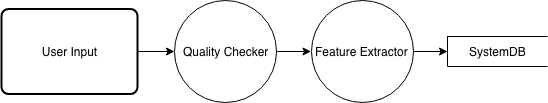
\includegraphics[width=\textwidth]{biometric_flowcharts-Enrolment.png}
	    \caption{Flowchart Showing User Enrolment In A Biometric System \citep{jain2004introduction}}
	    \label{fig:flowchat:enrolment}
	\end{figure}
	
		\begin{figure}[H]
	    \centering
	   % Make graphic fit page using \textwidth
	    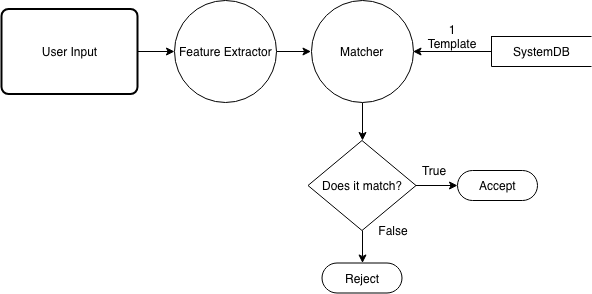
\includegraphics[width=\textwidth]{biometric_flowcharts-Verification.png}
	    \caption{Flowchart Showing User Verification In A Biometric System \citep{jain2004introduction}}
	    \label{fig:flowchat:verification}
	\end{figure}
	
		\begin{figure}[H]
	    \centering
	   % Make graphic fit page using \textwidth
	    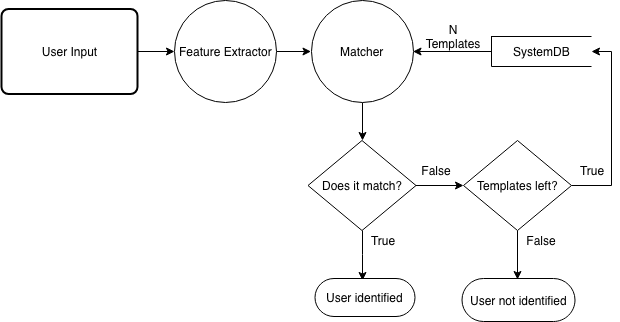
\includegraphics[width=\textwidth]{biometric_flowcharts-Identification.png}
	    \caption{Flowchart Showing User Identification In A Biometric System \citep{jain2004introduction}}
	    \label{fig:flowchat:identification}
	\end{figure}
	
	\subsection{Alternative Methods}
	Other methods of identification include the use of government issued documents such as drivers licences and passports.
	Trusona Inc. have developed a system that allows users to securely identify themselves with a physical ID card \citep{eisen2017systems}. Trusona has created authentication systems for the FBI \citep{abagnale_2017} thus highlighting how secure this technology can be. However this technology does have a significant barrier to entry, a user needs to have a physical form of identification in order to identify themselves on the system. In the cases of those who do not have documents such as passports, drivers licences or other forms of physical identification it would not be possible for them to use such a system.
	
	\subsection{Specific Methods}
	\label{subsect:specific_methods}
	\subsubsection{Fingerprints}
	\label{subsubsect:fingerprints}
	Fingerprint identification is widely used in smart phones such as Apple's iPhone and Samsung's S series of devices. Given it's wide use it's important that it is doesn't identify two different people as the same person, measured by \emph{false match rate} (FMR) \citep{delac2004survey}. The FMR of fingerprint identification has been observed as $0.2\%$ \citep{delac2004survey}. This is very low however the experiment only appears to include adults between the age of 20-39, excluding many younger and older people who also need access to fingerprint identification technology. It is not sufficient to include a subset of the population when discussing identification technology. Another issue with fingerprint technology is when user's do not have fingerprints. Fingerprint loss can occur through some medical treatments including chemotherapy \citep{al2012chemotherapy}. When it comes to smartphone authentication and identification technology it may be prudent to explore alternative biometric methods that are more universal with lower barriers to entry like face identification \citep{prabhakar2003biometric}.
	\\
	\\
	\subsubsection{Face Identification}
	\label{subsubsect:face_identification}
	As mentioned above face identification is now being introduced into Apple's new iPhone models (X, XS and XS Max). Traditionally face identification has suffered technological issues, specifically a lack of accuracy in ``environments with cluttered backgrounds and varied lighting conditions" \citep{prabhakar2003biometric}. Apple's \emph{``FaceID"} technology avoids this issue by projecting 30,000 infared dots onto the user's face to produce a sequence of depth maps and infared images \citep{apple_faceid_2017}. To further enhance security and avoid spoofing the sequences are randomised \citep{apple_faceid_2017}.
	\\
	\\
	\subsubsection{Handwriting Recognition}
	\label{subsubsect:handwriting_recognition}
	As a method of user identification handwriting recognition is arguably more accessible and useful today as opposed to before the advent of widespread, accurate touchscreen devices. There are two types of handwriting recognition: \emph{on-line} or \emph{dynamic} and \emph{off-line} or \emph{static} \citep{tappert_handwriting}. Off-line handwriting recognition is processed after a person has written something. For example a person may have written a letter on paper, this could then be analysed by a handwriting recognition system and the person's identity could be determined. Because identification does not happen in real-time off-line handwriting recognition is more suited to multi-factor authentication systems, where a user may provide one form of identification initially and then be required to support that initial identity challenge with an example of their handwriting. More useful today, perhaps, is on-line handwriting recognition, where a user may be identified as they are writing using a transducer \citep{tappert_handwriting}. This is of note given the large number of touchscreen devices such as phones, tablets and laptops that can be used as inputs to handwriting recognition systems.
	\\
	\\
	\subsubsection{Signature Recognition}
	\label{subsubsect:signature_recognition}
	Quite closely related to handwriting recognition (\ref{subsubsect:handwriting_recognition}) is signature recognition. Similar to handwriting recognition there are two methods of performing the identification, \emph{on-line} and \emph{off-line}. Signatures are already widely used in many aspects of people's lives, this reduces the barrier to entry as most people will already be used to signing documents and have standard way of doing it. It is also worth noting that people can find aspects of unfamiliar technology frightening and by using methods already familiar to people it may make user's feel more at ease with the system.
	
	There are issues with signature recognition, people are liable to change their signatures over a period of time and signatures are traditionally are liable to forgeries \citep{jain2004introduction}. These are substantial issues when attempting to securely identify a person. Variations make can make systems liable to false matches as two similar signatures with in-built variance may appear to be the same. Signature recognition is also liable to spoof-attacks \citep{jain2004introduction}. Traditional methods of signature forgery will still apply to signature recognition systems and, given that signature forgery has been used to defraud people for many years, it can be assumed that this practice will render signature recognition system insecure for identification over a network.
	\\
	\\
	\subsubsection{Keystroke Dynamics}
	\label{subsubsect:keystroke_dynamics}
	Given that one of the main inputs to most computer systems is a keyboard (either a software keyboard on a touchscreen or a hardware keyboard) it would be useful if one could be identified through it. Using features extracted from a user's typing, including time-features such as down-down times, down-up times, up-down times and the key code of the key typed by the user \citep{typing_auth2005}. These features in the system proposed in \cite{typing_auth2005} gave false rejection rates of $1.45\%$, false acceptance rates of $1.89\%$ for impostor users and false acceptance rates of $3.66\%$ for impostors that had observed legitimate users typing habit. This was proposed as an augmentation to traditional username \& password systems to make them more secure without requiring users to provide any further identification or any further effort.
	
	The features required may be difficult to legitimately collect, however. It is possible that software attempting to identify a user based on their typing habits may constitute key-logging which is in breach of many country's laws. A person's typing habits are also liable to change based on a number of external factors such as fatigue or simply the task one is engaged in. A person's typing will also improve over time as they become more accustomed to typing on a particular keyboard and thus the latency between key presses that the method above (and other methods such as \cite{shepherd_ibm_keystroke_auth1995}) focused on are liable to change.
	\\
	\\
	\subsubsection{Speaker Recognition}
	\label{subsubsect:speaker_recognition}
	Speaker recognition focuses on identifying a user based on characteristics of their speech. Two main versions of speaker recognition exist: \emph{text-dependent} and \emph{text-independent}. Text-dependent speaker recognition attempts to identify a speaker based on a particular phrase, whereas text-independent speaker recognition attempts to identify the speaker without the need for a specific utterance \citep{microsoft_2006}. In use cases where a user is already speaking, such as telephone banking, speaker recognition is incredibly useful and requires very little change in a user's behaviour. HSBC and other banks such as Citi have been using speaker recognition to identify their users since 2016 \citep{kollewe_2016}. Text-independent speaker recognition is more resistant to fraud \citep{jain2004introduction} but needs more training in order to perform well \citep{microsoft_2006}. Given that text-dependent speaker recognition requires a specific phrase be said, it could be combined with a password or PIN to enhance it's security.
	
	\section{Analysis and Discussion}
	\label{sect_analysis}
	\subsection{Comparison and Contrast}
	Many surveys display a table like Table \ref{tab:common_comparison} to compare and evaluate different biometrics in relation to their performance, security and usability.

    \begin{table}[H]
        \centering
        \begin{tabular}{|p{3cm}|p{2.5cm}|p{1.5cm}|p{2cm}|p{2cm}|p{2cm}|}
            \hline
             \textbf{Biometric} & \textbf{Fingerprint} & \textbf{Face} & \textbf{Hand Geometry} & \textbf{Iris} & \textbf{Voice} \\
             \hline
             \textbf{Barriers to universality} & Worn ridges; hand or finger impairment & None & Hand impairment & Visual impairment & Speech impairment \\\hline
             \textbf{Distinctiveness} & High & Low & Medium & High & Low\\\hline
             \textbf{Permanence} & High & Medium & Medium & High & Low\\\hline
             \textbf{Collectibility} & Medium & High & High & Medium & Medium\\\hline
             \textbf{Performance} & High & Low & Medium & High & Low \\\hline
             \textbf{Acceptability} & Medium & High & Medium & Low & High \\\hline
             \textbf{Potential for circumvention} & Low & High & Medium & Low & High \\\hline
        \end{tabular}
        \caption{Standard Biometric Comparison Table From: \cite{prabhakar2003biometric}}
        \label{tab:common_comparison}
    \end{table}
	
	This table can offer a good insight into which biometrics appear to be most effective, for example Fingerprints appear to be quite unique, quite permenant, fairly collectable and difficult to circumvent. This is likely why they are used in many consumer devices (such as mobile phones and some laptop computers). Compared to voice recognition it appears to be far better. Table \ref{tab:common_comparison} suggests voice recognition is not very distinct, liable to change and quite easy to circumvent.
	The issue with table \ref{tab:common_comparison} is that it only contains a handful of biometrics and the author (\cite{prabhakar2003biometric}) has not evaluated many behavioural biometrics such as handwriting recognition, signature recognition and keystroke dynamics.
	
	Another issue with table \ref{tab:common_comparison} is that it does not use numerical data to compare the different biometric methods. Most commonly when measuring biometric identification performance one measures ``the percentage of queries in which the correct answer can be found in the top few matches" \citep{phillips_evaluating_biometric_systems2000}. For verification one would measure the false-alarm rate and false-reject rate \citep{phillips_evaluating_biometric_systems2000}. The false-alarm rate measures a system's likelihood to accept an invalid identity whereas the false-reject rate measures a system's liklihood of rejecting a valid signature. When developing a system targets for the false-alarm and false-reject rate can be set. These depend on the application and thus may make comparing implementations difficult as one false-reject/false-alarm rate that may be ideal for a particular system or implementation could not be optimal for a different system or implementation \citep{phillips_evaluating_biometric_systems2000}. 
	
	In contrast to these measures \cite{TASSABEHJ_Evaluating_biometrics_for_online_banking2012} uses the System Usability Scale (SUS) \citep{brooke1996sus} to evaluate the usability of a biometric system designed for use in online banking. The article evaluates the usability of different biometric systems finding that fingerprint scanning was deemed favourable amongst users in terms of ease of use and security. While usability of the biometric system is important it could be argued that it's perceived merits are secondary to it's actual performance as a secure identification method and therefore the false-alarm and false-reject rates discussed previously are more important.
	
	\cite{phillips_evaluating_biometric_systems2000} gives guidance on how researchers should evaluate biometric systems. The article suggests researchers should:
	\begin{itemize}
	    \item Test on biometric signatures not yet seen by the system. To test on signatures the system has been trained with would simply result in assesing the ability to ``tune a system to a particular data set" \citep{phillips_evaluating_biometric_systems2000}.
	    \item Publish the evaluation procedure, evaluation protocols, examples from the data set and performance results \citep{phillips_evaluating_biometric_systems2000}.
	    \item Ensure the evaluation is not too hard or easy. If it is too easy or hard then the test will produce results that are not able to be compared to other tests \citep{phillips_evaluating_biometric_systems2000}.
	\end{itemize}
	
	When looking at evaluations of behavioural biometric systems many of the same measures that are used to evaluate biometric systems are presented. An example of this is \cite{typing_auth2005} which uses false-reject rates and false-accept (false-alarm) rates to evaluate a keystroke-dynamics based system. The evaluation also appears to mostly follow the suggestions outlined in \cite{phillips_evaluating_biometric_systems2000} 
	
	With the behavioural biometrics discussed in \ref{sect_methods} \& \ref{subsect:specific_methods} it is clear that there are distinct use cases for each. With regards to the internet and identifying a person online the use of keystroke dynamics to augment an existing username \& password system would enhance security whilst requiring very little extra effort on the part of the user. In cases where a user is already using their voice to interact with a system (smart speakers, telephone banking etc...) it would again add further security to an existing PIN or pass-phrase based identification system without the user being required to do anything more than enrolment.
	
	Whilst behavioural biometrics may not yet be secure and reliable enough to be used as a system's only form of identification they are certainly good candidates for use in multi-factor identification/authentication systems \citep{yampolskiy2008behavioural}.
	
	\subsection{Evaluation}
	\subsubsection{Comparison of Biometrics and Behavioural Biometrics}
	\label{subsubsect:biometric_behavioural_comparison}
	To compare biometric and behavioural biometric forms of identification and verification one should take into account not only the security but the impact on the user. With regards to the ethical implications of data collection it may impact users greatly if biometric features were accessed by a malicious third party. 
	
	Both the biometric and behavioural biometric fields contain more and less secure methods, however behavioural biometric systems tend to be less obtrusive with how they collect data \citep{yampolskiy2008behavioural}. While behavioural biometrics do not necessarily provide enough accuracy for identification, for verification purposes they appear to work well \citep{yampolskiy2008behavioural}, and certainly would be well suited to multi-factor authentication systems.
	
	\section{Summary}
	The use of biometrics and behavioural biometrics for user identification is already becoming widely used in modern technology. Services like Apple's TouchID and FaceID help popularise biometric forms of identification and help keep user's data more secure that if they were simply authenticated with usernames and passwords or a PIN. Behavioural biometric identification methods such as handwriting recognition (\ref{subsubsect:handwriting_recognition}), signature recognition (\ref{subsubsect:signature_recognition}), keystroke dynamics (\ref{subsubsect:keystroke_dynamics}) and speaker recognition (\ref{subsubsect:speaker_recognition}) can all be used to enhance the security of existing systems without requiring much more effort on the part of the user. This is important as user's are likely to reject new technology that overcomplicates a system they already deem to be secure enough.
	
	It is clear that usernames \& passwords are not secure enough when it comes to securing user's sensitive data. Failings in the username \& password system have been consistently highlighted through a number of high-profile data breaches and alternatives must be considered.
	
	While biometric identification methods may have issues of their own, it can be proven that they are more secure than usernames \& passwords and that they remove many of the issues that username \& password identification faces, such as susceptibility to brute-force attacks or bad decisions made by users.
	
	With the constant threat of security breaches it is imperative implementations of alternative identification methods be explored and considered. Username \& password based authentication is proven to be greatly flawed and should not be solely relied on.
	
	\bibliographystyle{agsm}
	\bibliography{references} 
	
\end{document}